\section{Sage}
\subsection{Un programa Sage con variables}

\begin{frame}
\frametitle{\insertsection}
\begin{block}{\insertsubsection}
\begin{itemize}
\item Es un sistema computarizado algebraico.
\item Utiliza el lenguaje de propósito general Python.
\item Creado por el matemático de la Universidad de Washington, William Stein, en el año 2005.
\item Sage reutiliza software libre existentes, algunos de ellos son GAP, PARI-GP, Maxima y Singular.
\item Está escrito completamente en Python.
\end{itemize}
\end{block}
\end{frame}

\begin{frame}[fragile]
\frametitle{\insertsection}
\begin{block}{\insertsubsection}
\begin{sageblock}
f(x) = exp(x) * sin(2*x)
\end{sageblock}
The second derivative of $f$ is

\[
\frac{\mathrm{d}^{2}}{\mathrm{d}x^{2}} \sage{f(x)} =
\sage{diff(f, x, 2)(x)}.
\]

Here's a plot of $f$ from $-1$ to $1$:
\end{block}

\begin{sagesilent}
plt  = plot(f, -1, 1)
plt.save("MyPic.pdf")
\end{sagesilent}

\begin{figure}
\centering
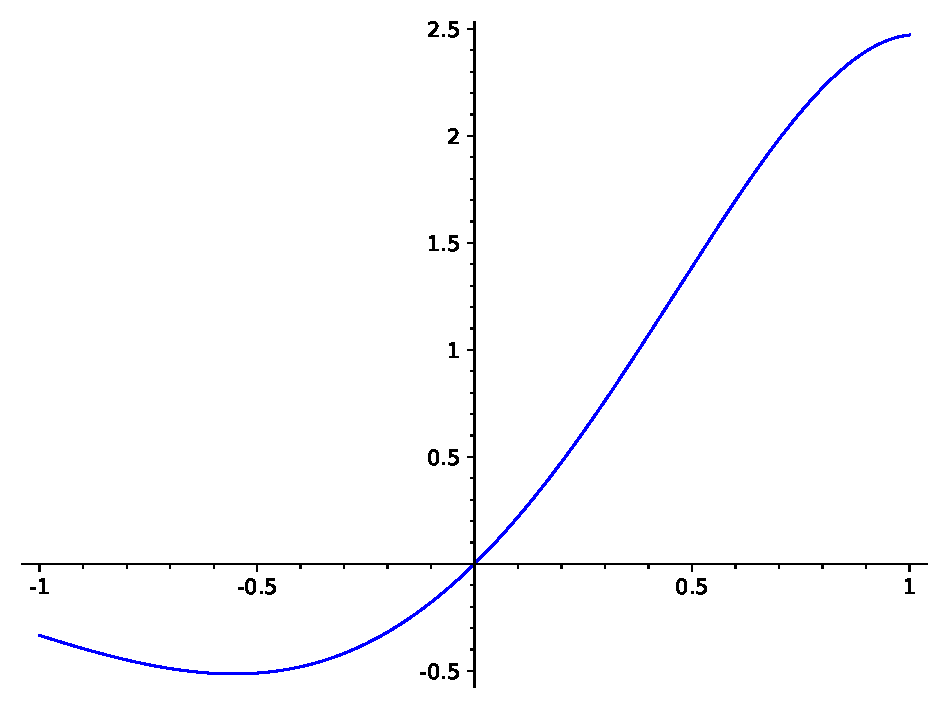
\includegraphics[height=3cm]{MyPic.pdf}
\end{figure}

\end{frame}

\begin{frame}
\begin{block}{Modelo matemático}
Nuestro primer ejemplo se refiere a la programación de un modelo matemático que predice la posición de una pelota lanzada al aire. De la segunda ley de Newton, y asumiendo que la resistencia del aire es insignificante, se puede derivar un modelo matemático que predice la posición $y$ de la pelota en el tiempo $t$.
\end{block}

La declaración $v_0$ = $5$ se llama \emph{asignación}
\end{frame}